\section{User Interfaces}\label{gui-sec}

A number of custom web applications were developed as part of the ETP. While many past Lean formalization projects have primarily relied on the Lean blueprint tool to organize tasks and track progress, the large volume of (transitive) implications tracked by the ETP, along with the research-oriented nature of the project, necessitated the development of custom tools to complement the blueprint tool. These web applications also made information more accessible to project participants and other interested parties, including those unfamiliar with Lean or the custom software developed for the project. The project features four primary interfaces:

\begin{enumerate}
  \item The \textbf{ETP dashboard}\footnote{\url{https://teorth.github.io/equational_theories/dashboard/}} displays the high-level overview of the project: the total number of resolved, conjectured, and unknown implications for the general and finite implication graphs. The dashboard also includes links to other tools, data, and visualizations about the implication graphs.
  \item The \textbf{Equation Explorer}\footnote{\url{https://teorth.github.io/equational_theories/implications/}} is the primary tool to navigate the implication graph. For a given equation, it display its inbound and outbound implications, as well as other members of its equivalence class. The explorer allows navigating either the general or finite implication graphs. The explorer also features custom commentary for a given equation (when available), serving as a repository for information and links. It also links to Graphiti visualizations and an example of its smallest satisfying magma, if one exists. Figure~\ref{fig:screenshot-equation-explorer} shows an example view of the explorer.
  \item \textbf{Graphiti}\footnote{\url{https://teorth.github.io/equational_theories/graphiti/}} visualizes the implication graph as a Hasse diagram, where downward edges represent subset relationships, and upward edges represent implications. Equivalence classes are collapsed into single nodes for clarity. Graphiti supports search parameters to visualize specific subsets of the graph. It can also display the entire implication graph, though the complete graph is large and challenging to navigate. Figure~\ref{fig:854-like} is an example of a Graphiti visualization.
  \item The \textbf{Finite Magma Explorer}\footnote{\url{https://teorth.github.io/equational_theories/fme/}} tests which equations a given finite magma satisfies or fails to satisfy. Users input finite magmas as Cayley tables. The tool is aware of the finite implication graph, so if an input magma witnesses an unknown refutation, it notifies the user and provides instructions for contributing the result to the GitHub repository.
\end{enumerate}

\begin{figure}
  \centering
  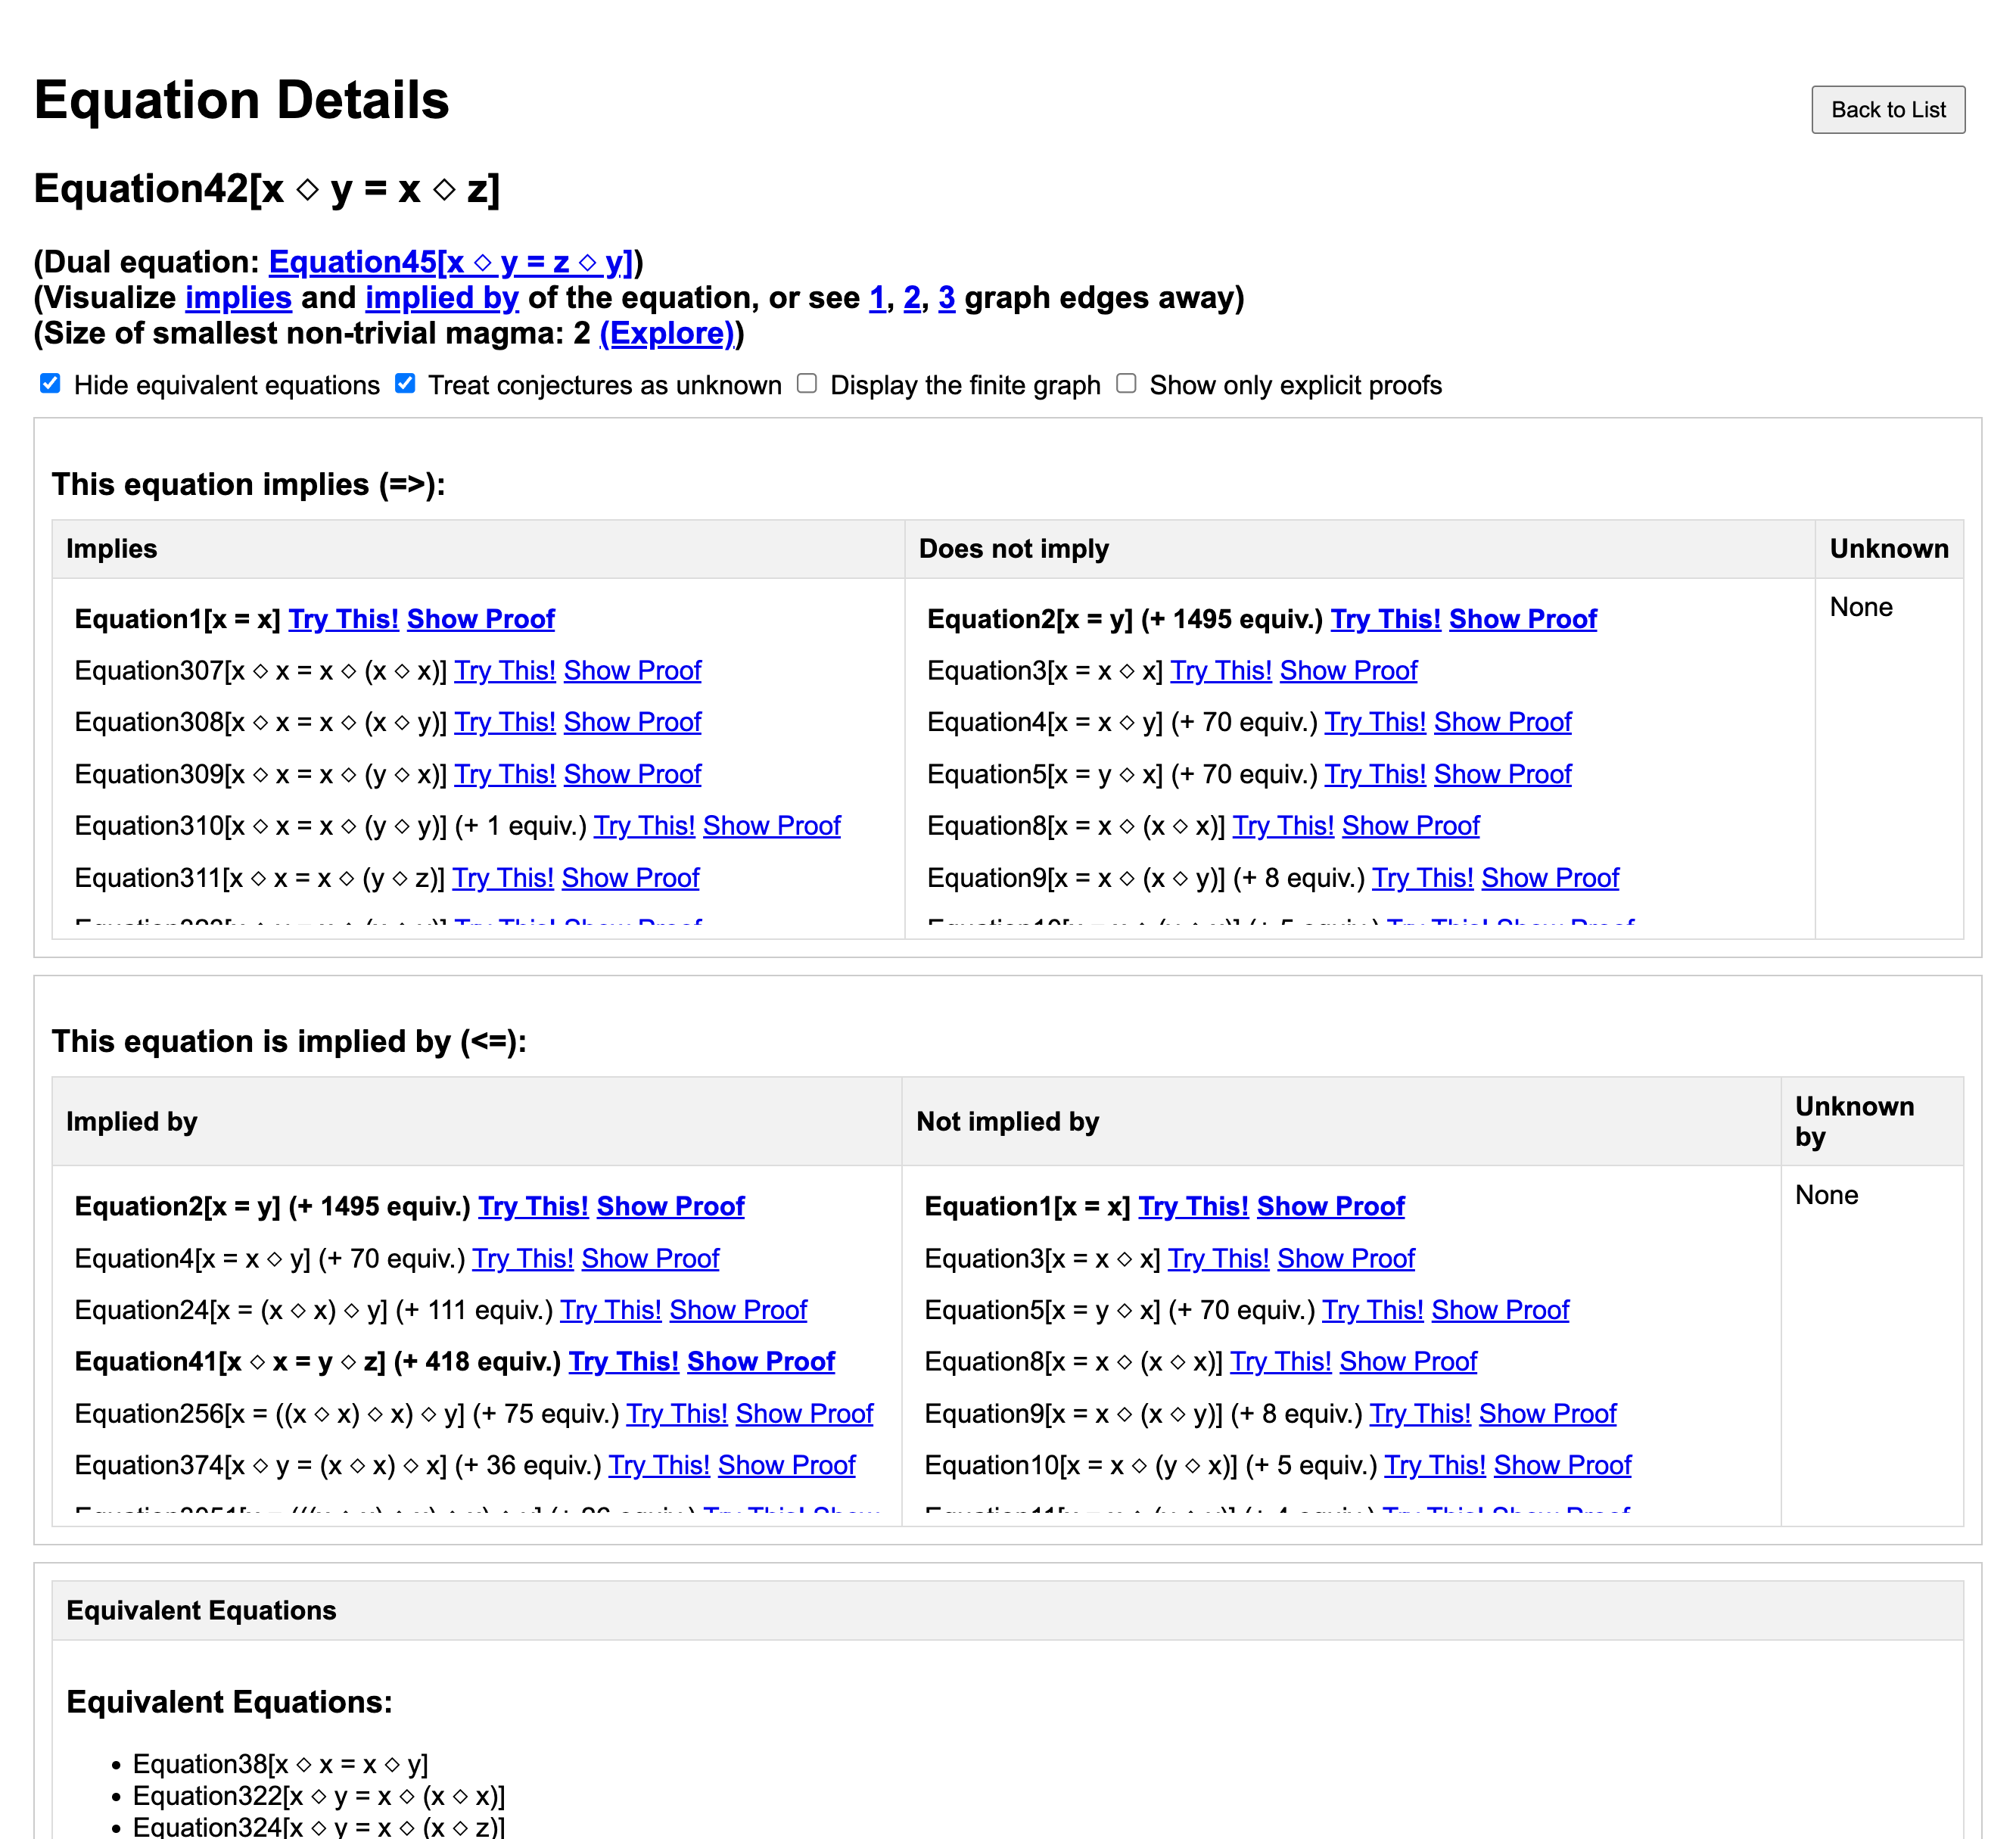
\includegraphics[width=0.85\textwidth]{GUI-equation-explorer.png}
  \caption{An example of the information displayed by the Equation Explorer for a specific equation.}
  \label{fig:screenshot-equation-explorer}
\end{figure}

The data for these tools is extracted directly from the Lean-formalized proofs in the project's GitHub repository, ensuring it always faithfully reflects the current state of progress. Additionally, the data is automatically updated with each code change using continuous integration (CI), eliminating the need for manual updates.
